\chapter{API Contracts Construction with Static Code Analysis}
\label{cha:codeAnalysis}

\section{Introduction}
\label{sec:contract-intro}
Code contracts are a concept derived from object-oriented principles in which preconditions, postconditions and invariants are defined for different software components. Specifically, the principle of ``design by contract'' suggests the use of specifications referred to as contracts. This provides a method for improving both code correctness and robustness as software components can only interact via obligations to contracts. Utilising this, we reduce the problem of linking API caveats to source code to the problem of mapping API caveats to code contracts. This allows us to simplify the problem of improving understanding of API caveat considerably by providing developers with immediate feedback while coding. Furthermore, finding a general method for transforming an arbitrary API caveat to a code contract is sufficient as we can assume the existence of programming analysis tools that can accept these contracts and locate patterns in source code (variations of such tools already exist). As a continuation of the previous chapter, I perform statistical analysis of several caveat types for the Java 12 API documentation based on work by \cite{zhou-directive}. I then propose a parsing technique to identify API caveats related to a significant subset of exceptions thrown and construct associated API contracts. This extends upon the parsing techniques used by \citeauthor{zhou-directive} to collect a subset of API caveats related to explicit constraints such as range limitations for arguments of a method, or not-null requirements. I propose and utilise an algorithm for analysing caveat sentences from this subset of API caveats to construct a total of 4,694 unique contracts. Finally, I develop a proof-of-concept checker plugin for IntelliJ that can be used to highlight violations of these API contracts in real time. \\

\section{Design}
\label{sec:contract-design}
The first step to generating contracts for API caveats is the extraction of API caveat sentences as described in \ref{subsec:info-caveat-extract}. We recall that caveat extraction using the approach described by \cite{caveat-knowledge-graph} on the Java 12 reference documentation yields 
115,243 caveat sentences, where a significant proportion of the sentences (67,701) are found within miscellaneous sections of an API element such as sentences in the parameters section for a method, or the description of a methods return value. Furthermore, we note that a subset of API caveats dealing with directives \cite{zhou-directive} contain explicit constraints that represent the largest portion (43.7\%) of API documentation \cite{directives-study}. From \cite{zhou-directive}, it can also be seen that a set of heuristic rules can be used to obtain constraints of type: (1) nullness not allowed, (2) nullness allowed, (3) type restriction and (4) range limitation from the directives of an API document. Although other categories of API caveats can also potentially be transformed into contracts and applied to static code analysis, I focus primarily on the categories identified by \cite{zhou-directive} for the scope of this project. \\

In addition, \cite{code-examples} proposes a method for mining API misuse by transforming source code to structure they refer to as API call sequences. These sequences essentially capture an API method call in addition to surrounding code elements such as guard conditions and method calls that are most relevant to the target API call. From this, we note that API contracts can be modified to apply to API call sequences given that contracts can be transformed to a structure resembling API call sequences.

\subsection{Java 12 Caveat Statistics Analysis}
\label{subsec:contract-caveat-statistics}
To better understand the prevalence of these API caveat categories identified by \cite{zhou-directive} in the Java 12 documentation, a statistical sampling method from \cite{singh2013elements} is applied. Specifically, the minimum number of samples required to ensure the estimated population mean is within a given confidence level and error margin can be calculated by the formula:

\begin{equation}
\label{sample}
min=\frac{\frac{z^2\times 0.25}{e^2}}{1 + \frac{(\frac{z^2\times 0.25}{e^2} - 1)}{p}}
\end{equation}

Where $z$ is the z-score associated with the desired confidence level, $e$ is the error margin and $p$ is the population size. For a 95\% confidence interval, 5\% error margin and a population size of 115,243 caveat sentences, the minimum sample size is approximately 383. However, we observe that the directive constraints identified by \cite{zhou-directive} correspond to the parameter and exception sections of method API elements specifically. This is because the directives they analysed were sentences annotated with \textit{@param, exception} and \textit{@throws} tags within the comments of the JDK source code files, which are transformed into HTML via Javadoc. It is also noted that the heuristic rules formulated by the authors for caveat categories of not-null, nullness allowed, type restriction and range limitation are differentiated for sentences with the \textit{@param} tag and for sentences with either \textit{@exception} or \textit{@throws} tags. Thus, we adopt a similar approach to reduce the scope of caveat sentences that require analysis. We specifically focus on the parameter or exception sections only API methods and constructors, and regard the sentences from those sections separately. \\

An observation on the parameter and exception sections of the Java 12 documentation is the consistent structure used for sentences. Sentences form the parameter section follow a template of ``\verb|param - description|'', where \verb|param| is the name of the parameter for a given method/constructor and \verb|description| is the actual sentence describing some information about \verb|param|. Exceptions also follow a similar template of ``\verb|exception - description|'', where \verb|exception| is the exception class thrown and \verb|description| describes conditions required for the exception to be thrown. An example of this is shown in Figure \ref{fig:api-doc-charAt}. It is therefore trivial to separate the \verb|description| sub-parts of a caveat sentence for analysis as we are only interested on the constraints imposed upon a particular parameter and the exception conditions. Moreover, we can filter the corpus of exception and parameter sentences to obtain a unique set of sentences for both as identical sentences can be mapped to the same contracts (but with different target parameters or API elements). Hence, two separate random samples of caveat sentences are collected: one from the parameters section of methods and constructors which consists of 2,654 unique sentences, and one from the exception sections of methods and constructors which consists of 4,870 unique sentences. Using equation \ref{sample}, the sample sizes required are 336 and 356 respectively. \\

\begin{figure}
	\label{fig:api-doc-charAt}
	\centering
	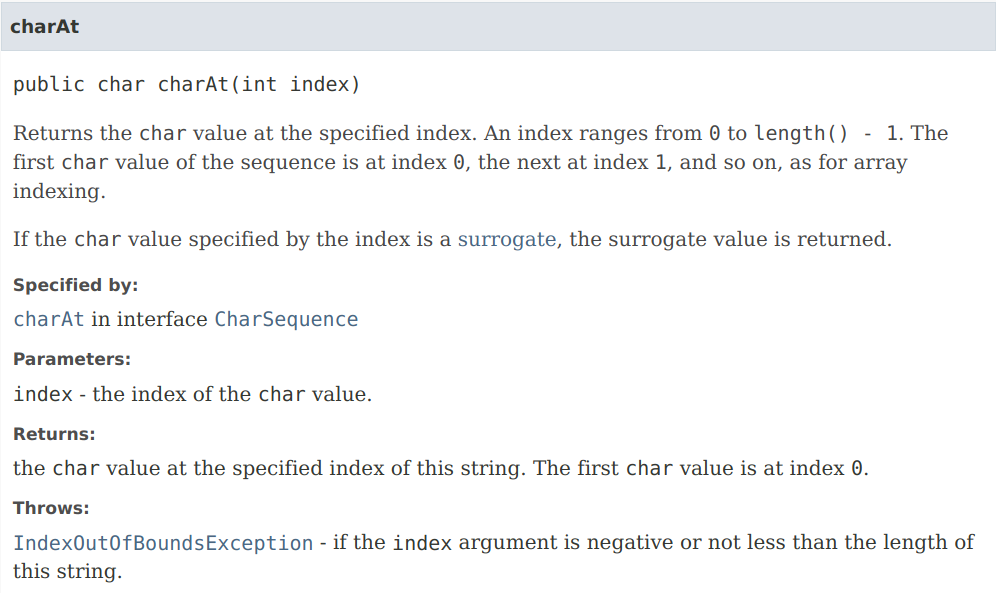
\includegraphics[width=0.75\textwidth]{figs/api-doc-charAt.png}
	\caption{API documentation for the \lstinline{charAt} method of the \lstinline{java.lang.String} class}
\end{figure}

Manual labelling is then required for the samples to identify the prevalence of different caveat types for the sentences. In  particular, the categories identified in \cite{zhou-directive} of \textit{not-null}, \textit{range limitation} and \textit{type restriction} are used as labels with the addition of \textit{ambiguous} to account for sentences that do not match any of the former classes. The \textit{not-null} category are defined as sentences which specify some parameter cannot be null. The \textit{range limitation} category specifies some numerical limitation on a parameter such as a non-negative requirement. Finally, the \textit{type restriction} category indicates that a parameter must a particular class type or one of several types. The \textit{nullness allowed} category is not considered from \cite{zhou-directive} because it only describes an acceptable condition for contracts, whereas the other categories describe a stricter condition for contracts that must not be broken. Overall, the results of this for the parameter sentences sample is shown in Table \ref{tab:caveat-param-stats}, while the results for exception level sentences is shown in Table \ref{tab:caveat-exception-stats}. We note that for \ref{tab:caveat-exception-stats}, the counts contribute add up to more than 356 because 6 of the labelled caveat samples fit both the \textit{not-null} category and the \textit{range limitation} category. 

\begin{table}[]
	\begin{tabular}{|l|cccc|}
		\hline
		& \multicolumn{4}{c|}{\textbf{Labels}} \\ \cline{2-5} 
		& \textbf{ambiguous} & \textbf{not-null} & \textbf{range limitation} & \textbf{type restriction} \\ \hline
		\textbf{Count} & 291 & 26 & 19 & 0 \\ \hline
	\end{tabular}
	\caption{Manually labelled results for classes of 336 randomly sampled parameter level caveat sentences.}
	\label{tab:caveat-param-stats}
\end{table}

\begin{table}[]
	\begin{tabular}{|l|cccc|}
		\hline
		& \multicolumn{4}{c|}{\textbf{Labels}} \\ \cline{2-5} 
		& \textbf{ambiguous} & \textbf{not-null} & \textbf{range limitation} & \textbf{type restriction} \\ \hline
		\textbf{Count} & 242 & 73 & 46 & 1 \\ \hline
	\end{tabular}
	\caption{Manually labelled results for classes of 356 randomly sampled exception level caveat sentences.}
	\label{tab:caveat-exception-stats}
\end{table}

From Table \ref{tab:caveat-param-stats}, it can be seen estimated that approximately 8\% of unique parameter caveat sentences impose a \textit{not-null} constraint and approximately 6\% of the unique parameter caveat sentences impose a \textit{range limitation} constraint. Despite the small percentage of sentences in parameter sentences sample that fit these categories, it its important to note that they represent one the most important type of API caveats: caveats that can cause software failures from exceptions. Furthermore, these caveat types are found to require (generally) explicit constraints that have little dependencies on other API elements, which makes them an adequate baseline for constructing code contracts. In contrast, the results from Table \ref{tab:caveat-exception-stats} show that considerably larger subset of 20\% of unique exception caveat sentences specify a \textit{non-null} constraint. This is also observed for the \textit{range limitation} category with approximately 13\% of sentences labelled. \\

Analysis of other categories must also be considered to determine what API contracts can be constructed and the approaches that are available. In particular, the categories identified in \cite{code-examples} are are derived from API misuse patterns data-mined from code snippets on Stack Overflow, but can be mapped into contracts. For example, \textit{missing control constructs} can be represented by an API contract that defines the control structure around some API call as a requirement. The same concept can also be applied to \textit{missing or incorrect order of API calls} and \textit{incorrect guard conditions}. However, it the subcategories of \textit{missing control constructs}, which include \textit{missing exception handling}, \textit{missing if checks} and \textit{missing finally}, all require explicit explanations for usage of these control structures. This is because usage of a control structure such as \lstinline{if} or \lstinline{finally} cannot be inferred without those keywords being described. Furthermore, \textit{incorrect guard conditions} could be considered a superset of the constraints analysed previously in \cite{zhou-directive} for the Java API documentation, but sentences that do not fit a category by \cite{zhou-directive} could then be expected to be rare occurrences. We therefore focus on \textit{missing control structures} and \textit{missing or incorrect order of API calls} as categories to analyse. Using a similar approach to before, the estimated sample size required is calculated with Equation \ref{sample} for sentences from the method/constructor description, parameter section or return value section, which are 321, 377, 336 and 353 respectively. The exception section sentences are not considered as they could all be categorised as descriptions of \textit{missing exception handling} or as examples of \textit{incorrect guard conditions}. In other words, all exception level sentences can be regarded as important, but extracting essential information from those sentences is non-trivial given their diversity. We therefore focus on a subset of these types of API caveats to reduce the scope of the project. The labelled results are shown in Table \ref{tab:caveat-sent-stats}. Note that \textit{Control} refers to \textit{missing control structures}, \textit{Temporal} refers to \textit{missing or incorrect order of API calls} and \textit{guard} refers to \textit{incorrect guard conditions}.\\

\begin{table}[]
	\begin{tabular}{|cc|cccc|}
		\hline
		&  & \multicolumn{4}{c|}{\textbf{Labels}} \\ \cline{3-6} 
		&  & \textbf{Ambiguous} & \textbf{Control} & \textbf{Temporal} & \textbf{Guard} \\ \hline
		\multicolumn{1}{|c|}{\multirow{4}{*}{\textbf{Sentence Location}}} & \textbf{Constructor} & 264 & 21 & 6 & 32 \\ \cline{2-6} 
		\multicolumn{1}{|c|}{} & \textbf{Method} & 360 & 9 & 4 & 5 \\ \cline{2-6} 
		\multicolumn{1}{|c|}{} & \textbf{Parameter} & 257 & 2 & 2 & 75 \\ \cline{2-6} 
		\multicolumn{1}{|c|}{} & \textbf{Return} & 351 & 0 & 1 & 0 \\ \hline
	\end{tabular}
	\caption{Manually labelled categories for caveat sentences found in different locations of the Java 12 API documentation.}
	\label{tab:caveat-sent-stats}
\end{table}

The results in Table \ref{tab:caveat-sent-stats} show the size of \textit{Control} and \textit{Temporal} caveat sentences is notably small, indicating that perhaps API documents rarely contain API methods that require specific call orders or additional control structures. This is an interesting result given that 31\% of 217,818 Stack Overflow posts studied in \cite{code-examples} were found to have a potential API misuse based on the categories mentioned previously. This suggests that API documentation may not contain sufficient information for developers to handle API caveats of these categories in particular.

\subsection{API Contracts Construction}
Given the results found from statistical analysis in \ref{subsec:contract-caveat-statistics}, the next step is to collect a set of API caveat sentences and attempt different approaches to extract important information for a given caveat. As a baseline study, the API caveats contained within the \textit{not-null} and \textit{range limitation} categories are the main caveats researched for this thesis. This is because the 64 heuristic rules and 29 regular expressions from \cite{zhou-directive} could be used as one approach for parsing an API caveat sentence. Their approach utilised these heuristics and regular expressions to parse the constraints of a caveat into a first-order logic (FOL) formula that can be passed to an satisfiability modulo theories (SMT) solver. However, their work (and the artefacts produced) are based on 429 documents of the JDK 1.8. In comparison to the Java 12 API documentation, 4,712 documents were data-crawled. Furthermore, large amounts of manual analysis is required to formulate these heuristic rules such that they can be generalised to multiple sentences for a given corpus. Hence, a simpler approach is proposed based on observations of the heuristics and some sample caveat sentences that are \textit{not-null} or \textit{range limitation} constraints. Thus, we can attempt to find a generalised approach for analysing sentences of these categories for different APIs and perhaps across other programming languages. \\

To design a simpler method for parsing API caveats with a \textit{not-null} constraint, we observe that sentences must mention the term ``null'' to either specify if a \lstinline{null} value is allowed or not allowed in code. Furthermore, given the structural information of the Java 12 API documentation, two notable sections already exist for each method/constructor of the API: the parameter list and exceptions list. These sections contain structural consistency in their sentences which follow a template described in \ref{subsec:contract-caveat-statistics}. Therefore, it is trivial to obtain information such as the subject of a sentence can obtained without the need for dependency parsing or part-of-speech (POS) tagging. Another observation made based on the heuristics from \cite{zhou-directive} is the prevalence of the subject-object-verb (SVO) ordering for a given sentence \cite{dryer200581}. Specifically, English is known to follow SVO ordering despite other possible logical orderings such as subject-object-verb used in Japanese or subject-verb-object in Mandarin. This structure can be seen from rules 1 and 17 of \ref{app:not-null}. For rule 20, we observe the use of ``non-null` as a predicative adjective to the subject, which is the only \textit{non-null} heuristic formulated that has ``null'' appearing before the subject. The final observation for this category of caveats is that whether some parameter for an API method call can be null is a boolean condition. In other words, this category of caveats represents the simplest form of an API contract as it only needs to specify whether a null value is accepted or disallowed for some dependent API element. Given this information, a general approach to identify whether an API caveat is of the \textit{non-null} category is to first filter for caveat sentences containing the sub-string ``null''. Next, we can assume that API documentations aim to be simplistic and mentions of nullness within certain sections (i.e. exception sections) can be regarded as a ``nullness not allowed'' constraint. This is particularly true for the Java API documentation as the sentences in exception sections of methods/constructors is used to describe the conditions required for the relevant exception to be thrown. Hence, any mention of ``null'' inside this section could be assumed to indicate a null value will result in an exception. We do note however that this assumption does not necessarily hold for other API documentation. \\

\begin{table}[]
	\begin{tabular}{|cc|}
		\hline
		Rule Number & Heuristic \\ \hline
		1 & [something] be/equals null \\
		17 & Value of [something] be/equals null \\
		20 & Non-null [something] \\ \hline
	\end{tabular}
	\caption{Example of 3 of 20 heuristic rules for nullness not allowed from \cite{zhou-directive}. Note that the complete list can be found in \ref{tab:not-null-heuristic} (Appendix).}
	\label{tab:not-null-heuristic}
\end{table}

\begin{table}[]
	\begin{tabular}{|cc|}
		\hline
		Rule Number & Heuristic \\ \hline
		1 & [something] >/</= [value] \\
		8 & [something] be {not} negative/positive/false/true \\
		20 & [something1] equals [something2] \\ \hline
	\end{tabular}
	\caption{Example of 3 of 23 heuristic rules for range limitations from \cite{zhou-directive}. Note that the complete list can be found in \ref{tab:range-limit-heuristic} (Appendix).}
	\label{tab:range-limit-heuristic}
\end{table}

An alternative approach for parsing the \textit{non-null} and \textit{range limitation} API caveats is to utilise a sentence normalisation technique used in \cite{zhou-directive}. In particular, several regular expressions are identified by \citeauthor{zhou-directive} to perform substitutions within a sentence prior to dependency parsing. These expressions are used to detect cases such as the names of variables, classes and mathematical expressions

% Please add the following required packages to your document preamble:
% \usepackage{multirow}
\begin{table}[]
	\begin{tabular}{|l|l|l|}
		\hline
		\textbf{Type} & \textbf{Description} & \textbf{Regular Expression} \\ \hline
		\multirow{2}{*}{Specific Values} & 0.0, 0.1f, etc. & \textbackslash{}W(-)?{[}0-9{]}+(,{[}0-9{]}+)*((\textbackslash{}.{[}0-9{]}+)?{[}a-z{]}*)\textbackslash{}W \\ \cline{2-3} 
		& \begin{tabular}[c]{@{}l@{}}Member value of objects \\ e.g., Location.x\end{tabular} & \textbackslash{}W(\textasciicircum{}(java\textbackslash{}.|javax\textbackslash{}.|org\textbackslash{}.))?({[}A-Za-z\_{]}+\textbackslash{}w+\textbackslash{}.)+{[}a-z\_{]}+{[}a-z0-9\_{]}*{[}\textasciicircum{}\textbackslash{}.A-Za-z0-9\_{]} \\ \hline
		\multirow{4}{*}{Class methods and static members} & \begin{tabular}[c]{@{}l@{}}class methods,\\ e.g., ClassA.func(Param1)\end{tabular} & \textbackslash{}W{[}A-Za-z\_{]}+{[}A-Za-z\_0-9{]}*(\textbackslash{}.{[}A-Za-z\_{]}+{[}A-Za-z\_0-9{]})*(\#{[}A-Za-z\_{]}+{[}A-Za-z\_0-9{]}*)?\([^()]*\)\textbackslash{}W \\ \cline{2-3} 
		& Static member, e.g.,  Desktop.Action\#OPEN & \textbackslash{}W({[}A-Za-z\_{]}+{[}A-Za-z\_0-9{]}*(\textbackslash{}.{[}A-Za-z\_{]}+{[}A-Za-z\_0-9{]})*)?(\#{[}A-Za-z\_{]}+{[}A-Za-z\_0-9{]}*){[}\textasciicircum{}A-Za-z0-9\_(){]} \\ \cline{2-3} 
		& All upper case & \textbackslash{}W(\textbackslash{}w+\textbackslash{}.)*({[}A-Z{]}+\_)*{[}A-Z{]}+\textbackslash{}W \\ \cline{2-3} 
		& Class name & \textbackslash{}W({[}A-Za-z\_{]}+\textbackslash{}w+\textbackslash{}.)*{[}A-Za-z\_{]}*{[}A-Z{]}+\textbackslash{}w+{[}\textasciicircum{}\textbackslash{}.A-Za-z0-9\_{]} \\ \hline
		\multirow{11}{*}{Expressions} & A - B & \textbackslash{}W\textbackslash{}w+((\textbackslash{}s+-)|(-\textbackslash{}s+)|(\textbackslash{}s+-\textbackslash{}s+))\textbackslash{}w+\textbackslash{}W \\ \cline{2-3} 
		& A + B & \textbackslash{}W\textbackslash{}w+\textbackslash{}s*\textbackslash{}+\textbackslash{}s*\textbackslash{}w+\textbackslash{}W \\ \cline{2-3} 
		& A * B & \textbackslash{}W\textbackslash{}w+\textbackslash{}s*\textbackslash{}*\textbackslash{}s*\textbackslash{}w+\textbackslash{}W \\ \cline{2-3} 
		& A..B & \textbackslash{}W(?\textbackslash{}s*\textbackslash{}w+\textbackslash{}s*)?\textbackslash{}s*\textbackslash{}.\textbackslash{}s*\textbackslash{}.\textbackslash{}s*(?\textbackslash{}s*\textbackslash{}w+\textbackslash{}s*)?\textbackslash{}W \\ \cline{2-3} 
		& {[}A, B{]} & \textbackslash{}W[\textbackslash{}s*\textbackslash{}w+\textbackslash{}s*,\textbackslash{}s*\textbackslash{}w+\textbackslash{}s*]\textbackslash{}W \\ \cline{2-3} 
		& {[}A..B{]} & \textbackslash{}W[\textbackslash{}s*\textbackslash{}w+\textbackslash{}s*(\textbackslash{}.\textbackslash{}s*\textbackslash{}.\textbackslash{}s*)\textbackslash{}s*\textbackslash{}w+\textbackslash{}s*]\textbackslash{}W \\ \cline{2-3} 
		& A \textless{}\textbackslash{}\textless{}= B \textless{}\textbackslash{}\textless{}= C & \textbackslash{}W\textbackslash{}w+\textbackslash{}s*\&lt;=?\textbackslash{}s*\textbackslash{}w+\textbackslash{}s*\&lt;=?\textbackslash{}s*\textbackslash{}w+\textbackslash{}W \\ \cline{2-3} 
		& A \textgreater{}\textbackslash{}\textgreater{}= B \textgreater{}\textbackslash{}\textgreater{}= C & \textbackslash{}W\textbackslash{}w+\textbackslash{}s*\&gt;=?\textbackslash{}s*\textbackslash{}w+\textbackslash{}s*\&gt;=?\textbackslash{}s*\textbackslash{}w+\textbackslash{}W \\ \cline{2-3} 
		& From A to B & \textbackslash{}W(from\textbackslash{}s+)?\textbackslash{}w+\textbackslash{}s+to\textbackslash{}s+\textbackslash{}w+\textbackslash{}W \\ \cline{2-3} 
		& A != B & \textbackslash{}W\textbackslash{}w+\textbackslash{}s*!=\textbackslash{}s*\textbackslash{}w+\textbackslash{}W \\ \cline{2-3} 
		& Enumeration expression & \textbackslash{}W (\textbackslash{}s*\textbackslash{}w+\textbackslash{}s*)(,\textbackslash{}s*\textbackslash{}w+\textbackslash{}s*)+,?\textbackslash{}s*or\textbackslash{}s*\textbackslash{}w+\textbackslash{}W \\ \hline
	\end{tabular}
	\caption{The regular expressions identified in \textbackslash{}cite\{\} for sub-sentence substitutions and dependency parsing.}
	\label{tab:zhou-regex}
\end{table}

\subsection{Checker Programs}
\fix{Describe IntelliJ plugin and Boa AST}

\section{Implementation}
\label{sec:contract-implement}

\subsection{Java API Caveat Contracts}
\label{subsec:contract-caveat-contracts}
\fix{Describe contract construction in Python}

\subsection{IntelliJ Plugin with Static Code Analysis}
\label{subsec:contract-plugin}
\fix{Explain IntelliJ plugin and Boa AST code}

\subsection{Boa Programming Language \& API Call Sequence Mining}
\label{subsec:contract-boa}
\fix{Maybe remove this section if it doesn't add much}

\section{Results}
\label{sec:contract-results}

\fix{Add screenshots of the IntelliJ plugin and table of results for potential errors from Boa}

\section{Summary}
\label{sec:contract-summary}
Same as the last chapter, summary what you discussed in this chapter and
be the bridge to next chapter.
